\documentclass{standalone}
% 

% \pgfmathdeclarefunction{gauss}{2}{%
%   \pgfmathparse{1/(#2*sqrt(2*pi))*exp(-((x-#1)^2)/(2*#2^2))}%
% }
\usepackage{tkz-euclide}
\usetkzobj{all}
\renewcommand{\familydefault}{\sfdefault}
\usepackage{calc,tikz}
\usetikzlibrary{calc}
\usepackage{pgfplots}
\begin{document}
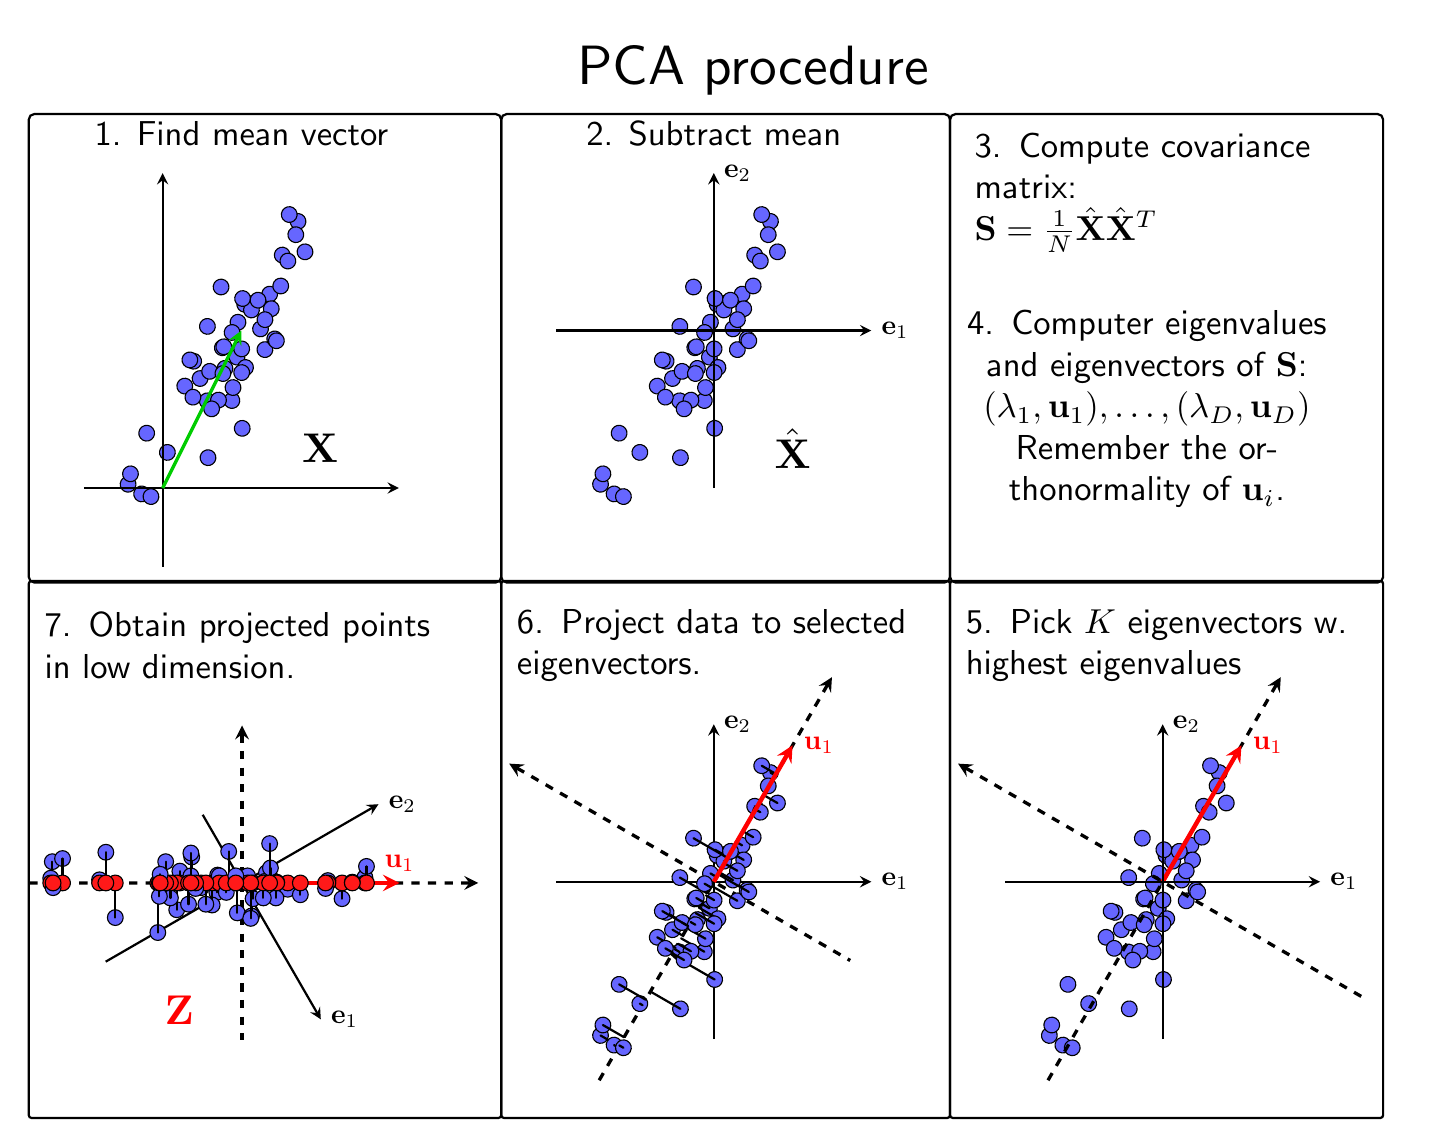
\begin{tikzpicture}[>=stealth]
    \def\normaltwo{\x,{4*1/exp(((\x-0)^2)/2)}}
    \node [scale = 2] at (6.5, 3.3) {PCA procedure};
    %%%%%%%%% block 1%%%%%%%%%%%%%%%%%
    \begin{scope}
        \draw [rounded corners = 2pt, thick] (-2.7, -3.2) rectangle (3.3, 2.75);
        \begin{scope}[rotate = 60]
            \foreach \x/\y/\z in {-0.32/-0.12/0, -0.06/-0.38/1, 1.27/-0.20/2, -0.31/0.10/3, 0.58/-0.08/4, -0.79/0.15/5, 0.31/0.13/6, -0.99/-0.07/7, 0.38/0.04/8, 0.12/-0.42/9, 0.07/0.09/10, 1.09/0.03/11, 0.29/0.02/12, -0.17/0.40/13, 0.36/0.19/14, 0.14/-0.20/15, -0.38/-0.28/16, -1.61/-0.44/17, -0.52/-0.06/18, 0.43/-0.19/19, 1.56/0.07/20, 1.58/0.21/21, -0.83/-0.34/22, 0.27/-0.19/23, -0.29/0.09/24, -2.41/0.27/25, -2.28/0.31/26, -0.20/-0.12/27, -0.64/0.33/28, 1.06/-0.07/29, -0.91/-0.19/30, -0.65/0.09/31, -0.68/-0.27/32, -1.07/-0.63/33, -2.43/0.06/34, -0.97/0.27/35, 1.40/0.01/36, -0.46/-0.27/37, 0.11/-0.45/38, -0.08/0.09/39, -1.81/0.04/40, 0.44/0.01/41, -2.40/-0.06/42, 0.74/-0.15/43, -1.05/-0.17/44, -0.59/-0.07/45, -0.65/0.38/46, 0.35/0.50/47, -1.73/0.39/48, -1.04/0.11/49} {
                \draw [fill = blue!60] (\x, \y) circle (1mm); }
        \end{scope}
        \draw[->, thick] (-2,-2) -- (2,-2) node[right] {};
        \draw[->, thick] (-1,-3) -- (-1,2) node[right] {};
        \draw[->, green!80!black, very thick] (-1, -2) --(0, 0) node[right] {};
        \node [scale = 1.5] at (1, -1.5) {$\mathbf{X}$};
        \node [scale = 1.25] at (0, 2.5) {1. Find mean vector};
    \end{scope}

    %%%%%%%%%% block 2 %%%%%%%%%%%%%%%%%%%
    \begin{scope}[xshift = 6cm]
        \draw [rounded corners = 2pt, thick] (-2.7, -3.2) rectangle (3, 2.75);
        \begin{scope}[rotate = 60]
            \foreach \x/\y/\z in {-0.32/-0.12/0, -0.06/-0.38/1, 1.27/-0.20/2, -0.31/0.10/3, 0.58/-0.08/4, -0.79/0.15/5, 0.31/0.13/6, -0.99/-0.07/7, 0.38/0.04/8, 0.12/-0.42/9, 0.07/0.09/10, 1.09/0.03/11, 0.29/0.02/12, -0.17/0.40/13, 0.36/0.19/14, 0.14/-0.20/15, -0.38/-0.28/16, -1.61/-0.44/17, -0.52/-0.06/18, 0.43/-0.19/19, 1.56/0.07/20, 1.58/0.21/21, -0.83/-0.34/22, 0.27/-0.19/23, -0.29/0.09/24, -2.41/0.27/25, -2.28/0.31/26, -0.20/-0.12/27, -0.64/0.33/28, 1.06/-0.07/29, -0.91/-0.19/30, -0.65/0.09/31, -0.68/-0.27/32, -1.07/-0.63/33, -2.43/0.06/34, -0.97/0.27/35, 1.40/0.01/36, -0.46/-0.27/37, 0.11/-0.45/38, -0.08/0.09/39, -1.81/0.04/40, 0.44/0.01/41, -2.40/-0.06/42, 0.74/-0.15/43, -1.05/-0.17/44, -0.59/-0.07/45, -0.65/0.38/46, 0.35/0.50/47, -1.73/0.39/48, -1.04/0.11/49} {
            \draw [fill = blue!60] (\x, \y) circle (1mm); }
        \end{scope}
        \draw[->, thick] (-2,0) -- (2,0) node[right] {$\mathbf{e}_1$};
        \draw[->, thick] (-0,-2) -- (-0,2) node[right] {$\mathbf{e}_2$};
        \node [scale = 1.5] at (1, -1.5) {$\hat{\mathbf{X}}$};
        \node [scale = 1.25] at (0, 2.5) {2. Subtract mean};
    \end{scope}

    %%%%%%%%%% block 3 %%%%%%%%%%%%%%%%%%%
    \begin{scope}[xshift = 9cm]
        \draw [rounded corners = 2pt, thick] (0, -3.2) rectangle (5.5, 2.75);
        \node [text width = 3.5cm, align = left, scale = 1.25] at (2.5, 1.75) {3. Compute covariance matrix: \\ $\mathbf{S} = \frac{1}{N}\hat{\mathbf{X}}\hat{\mathbf{X}}^T$};

        \node [text width = 5cm, align = center, scale = 1.25] at (2.5, -1) {4. Computer eigenvalues and eigenvectors of $\mathbf{S}$: \\ $ (\lambda_1, \mathbf{u}_1), \dots, (\lambda_D, \mathbf{u}_D)$\\ Remember the orthonormality of $\mathbf{u}_i$.};
    \end{scope}

    %%%%%%%%%% block 4 %%%%%%%%%%%%%%%%%%%
    \begin{scope}[xshift = 11.7cm, yshift = -7cm]
        \draw [rounded corners = 1pt, thick] (-2.7, -3) rectangle (2.8, 3.82);
        \begin{scope}[rotate = 60]
                \foreach \x/\y/\z in {-0.32/-0.12/0, -0.06/-0.38/1, 1.27/-0.20/2, -0.31/0.10/3, 0.58/-0.08/4, -0.79/0.15/5, 0.31/0.13/6, -0.99/-0.07/7, 0.38/0.04/8, 0.12/-0.42/9, 0.07/0.09/10, 1.09/0.03/11, 0.29/0.02/12, -0.17/0.40/13, 0.36/0.19/14, 0.14/-0.20/15, -0.38/-0.28/16, -1.61/-0.44/17, -0.52/-0.06/18, 0.43/-0.19/19, 1.56/0.07/20, 1.58/0.21/21, -0.83/-0.34/22, 0.27/-0.19/23, -0.29/0.09/24, -2.41/0.27/25, -2.28/0.31/26, -0.20/-0.12/27, -0.64/0.33/28, 1.06/-0.07/29, -0.91/-0.19/30, -0.65/0.09/31, -0.68/-0.27/32, -1.07/-0.63/33, -2.43/0.06/34, -0.97/0.27/35, 1.40/0.01/36, -0.46/-0.27/37, 0.11/-0.45/38, -0.08/0.09/39, -1.81/0.04/40, 0.44/0.01/41, -2.40/-0.06/42, 0.74/-0.15/43, -1.05/-0.17/44, -0.59/-0.07/45, -0.65/0.38/46, 0.35/0.50/47, -1.73/0.39/48, -1.04/0.11/49 }
                {\draw [fill = blue!60] (\x, \y) circle (1mm); }
        \end{scope}
        \draw [<-, very thick, dashed] ($(0,0) + (60:3)$) -- ($(0,0) + (240:3)$);
        \draw [<-, very thick, dashed] ($(0,0) + (150:3)$) -- ($(0,0) + (-30:3)$);
        \draw[->, ultra thick, red] (0, 0) -- ($(0,0) + (60:2)$) node[right] {$\mathbf{u}_1$};
        \draw[->, thick] (-2,0) -- (2,0) node[right] {$\mathbf{e}_1$};
        \draw[->, thick] (-0,-2) -- (-0,2) node[right] {$\mathbf{e}_2$};
        \node [scale = 1.25, text width = 4cm] at (0, 3) {5. Pick $K$ eigenvectors w. highest eigenvalues};
    \end{scope}

    %%%%%%%%%% block 5 %%%%%%%%%%%%%%%%%%%
    \begin{scope}[xshift = 6cm, yshift = -7cm]
        \draw [rounded corners = 1pt, thick] (-2.7, -3) rectangle (3, 3.82);
        \node [scale = 1.25, text width = 4cm] at (0, 3) {6. Project data to selected eigenvectors.};

        \tkzDefPoint(60:3){A}
        \tkzDefPoint(240:3){B}
        \draw [<-, very thick, dashed] (A) -- (B);
        \draw [<-, very thick, dashed] ($(0,0) + (150:3)$) -- ($(0,0) + (-30:2)$);
        \draw[->, thick] (-2,0) -- (2,0) node[right] {$\mathbf{e}_1$};
        \draw[->, thick] (-0,-2) -- (-0,2) node[right] {$\mathbf{e}_2$};

        
        \begin{scope}[rotate = 60]
            \foreach \x/\y/\z in {-0.32/-0.12/0, -0.06/-0.38/1, 1.27/-0.20/2, -0.31/0.10/3, 0.58/-0.08/4, -0.79/0.15/5, 0.31/0.13/6, -0.99/-0.07/7, 0.38/0.04/8, 0.12/-0.42/9, 0.07/0.09/10, 1.09/0.03/11, 0.29/0.02/12, -0.17/0.40/13, 0.36/0.19/14, 0.14/-0.20/15, -0.38/-0.28/16, -1.61/-0.44/17, -0.52/-0.06/18, 0.43/-0.19/19, 1.56/0.07/20, 1.58/0.21/21, -0.83/-0.34/22, 0.27/-0.19/23, -0.29/0.09/24, -2.41/0.27/25, -2.28/0.31/26, -0.20/-0.12/27, -0.64/0.33/28, 1.06/-0.07/29, -0.91/-0.19/30, -0.65/0.09/31, -0.68/-0.27/32, -1.07/-0.63/33, -2.43/0.06/34, -0.97/0.27/35, 1.40/0.01/36, -0.46/-0.27/37, 0.11/-0.45/38, -0.08/0.09/39, -1.81/0.04/40, 0.44/0.01/41, -2.40/-0.06/42, 0.74/-0.15/43, -1.05/-0.17/44, -0.59/-0.07/45, -0.65/0.38/46, 0.35/0.50/47, -1.73/0.39/48, -1.04/0.11/49 } {

                \tkzDefPoint(\x, \y){x\z}
                \draw [fill = blue!60] (\x, \y) circle (1mm); 
                \tkzDefPointBy[projection=onto B--A](x\z)
                \tkzGetPoint{H\z}
                \tkzDrawLines[add = 0 and 0, thick](x\z,H\z)

                }
        \end{scope}
        \draw[->, ultra thick, red] (0, 0) -- ($(0,0) + (60:2)$) node[right] {$\mathbf{u}_1$};
    \end{scope}

    %%%%%%%%%% block 6 %%%%%%%%%%%%%%%%%%%
    \node [scale = 1.25, text width = 4cm] at (0, -4) {7. Obtain projected points in low dimension.};
    \begin{scope}[xshift = 0cm, yshift = -7cm]
        \draw [rounded corners = 1pt, thick] (-2.7, -3) rectangle (3.3, 3.82);
    \begin{scope}[rotate = -60, xshift = .5]
        \tkzDefPoint(60:3){A}
        \tkzDefPoint(240:2.7){B}
        \draw [<-, very thick, dashed] (A) -- (B);
        \draw [<-, very thick, dashed] ($(0,0) + (150:2)$) -- ($(0,0) + (-30:2)$);
        \draw[->, ultra thick, red] (0, 0) -- ($(0,0) + (60:2)$) node[above] {$\mathbf{u}_1$};
        % \draw[->, ultra thick, red] (0, 0) -- ($(0,0) + (150:2)$) node[right] {$\mathbf{u}_2$};
        \draw[->, thick] (-1,0) -- (2,0) node[right] {$\mathbf{e}_1$};
        \draw[->, thick] (-0,-2) -- (-0,2) node[right] {$\mathbf{e}_2$};


        \begin{scope}[rotate = 60]
            \foreach \x/\y/\z in {-0.32/-0.12/0, -0.06/-0.38/1, 1.27/-0.20/2, -0.31/0.10/3, 0.58/-0.08/4, -0.79/0.15/5, 0.31/0.13/6, -0.99/-0.07/7, 0.38/0.04/8, 0.12/-0.42/9, 0.07/0.09/10, 1.09/0.03/11, 0.29/0.02/12, -0.17/0.40/13, 0.36/0.19/14, 0.14/-0.20/15, -0.38/-0.28/16, -1.61/-0.44/17, -0.52/-0.06/18, 0.43/-0.19/19, 1.56/0.07/20, 1.58/0.21/21, -0.83/-0.34/22, 0.27/-0.19/23, -0.29/0.09/24, -2.41/0.27/25, -2.28/0.31/26, -0.20/-0.12/27, -0.64/0.33/28, 1.06/-0.07/29, -0.91/-0.19/30, -0.65/0.09/31, -0.68/-0.27/32, -1.07/-0.63/33, -2.43/0.06/34, -0.97/0.27/35, 1.40/0.01/36, -0.46/-0.27/37, 0.11/-0.45/38, -0.08/0.09/39, -1.81/0.04/40, 0.44/0.01/41, -2.40/-0.06/42, 0.74/-0.15/43, -1.05/-0.17/44, -0.59/-0.07/45, -0.65/0.38/46, 0.35/0.50/47, -1.73/0.39/48, -1.04/0.11/49 } {

                \tkzDefPoint(\x, \y){x\z}
                \draw [fill = blue!60] (\x, \y) circle (1mm); 
                \tkzDefPointBy[projection=onto B--A](x\z)
                \tkzGetPoint{H\z}
                \tkzDrawLines[add = 0 and 0, thick](x\z,H\z)
                \draw [fill = red!90] (H\z) circle (1mm); 

                }
        \end{scope}
        \node [scale = 1.5, red] at (1, -1.5) {$\mathbf{Z}$};
    \end{scope}
    \end{scope}


    

\end{tikzpicture}
\end{document}